\begin{center}
\vspace{1cm}
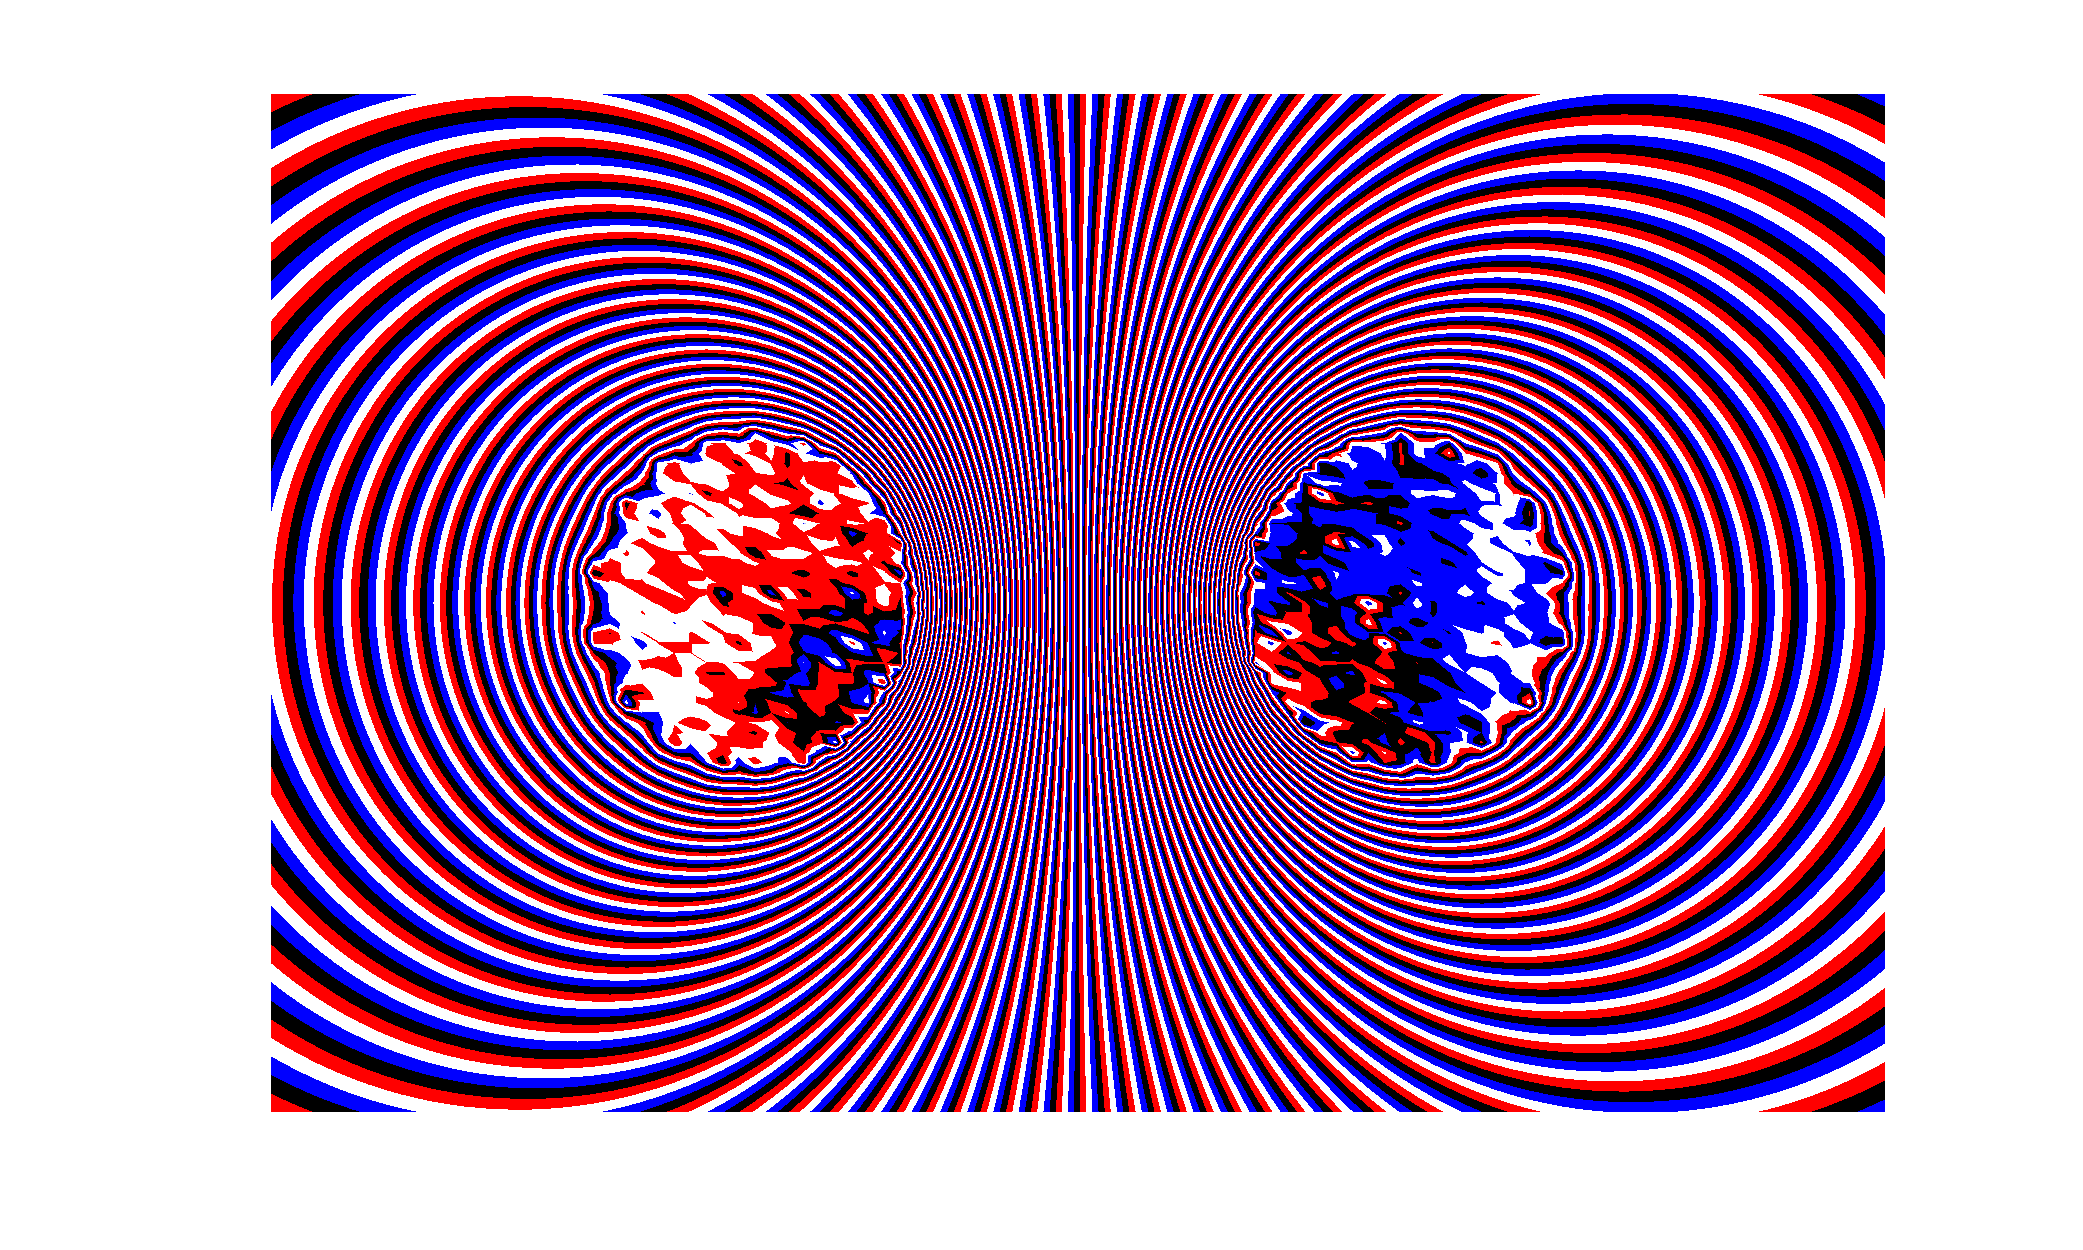
\includegraphics[width=.45\textwidth]{figures/art/1a_2D}
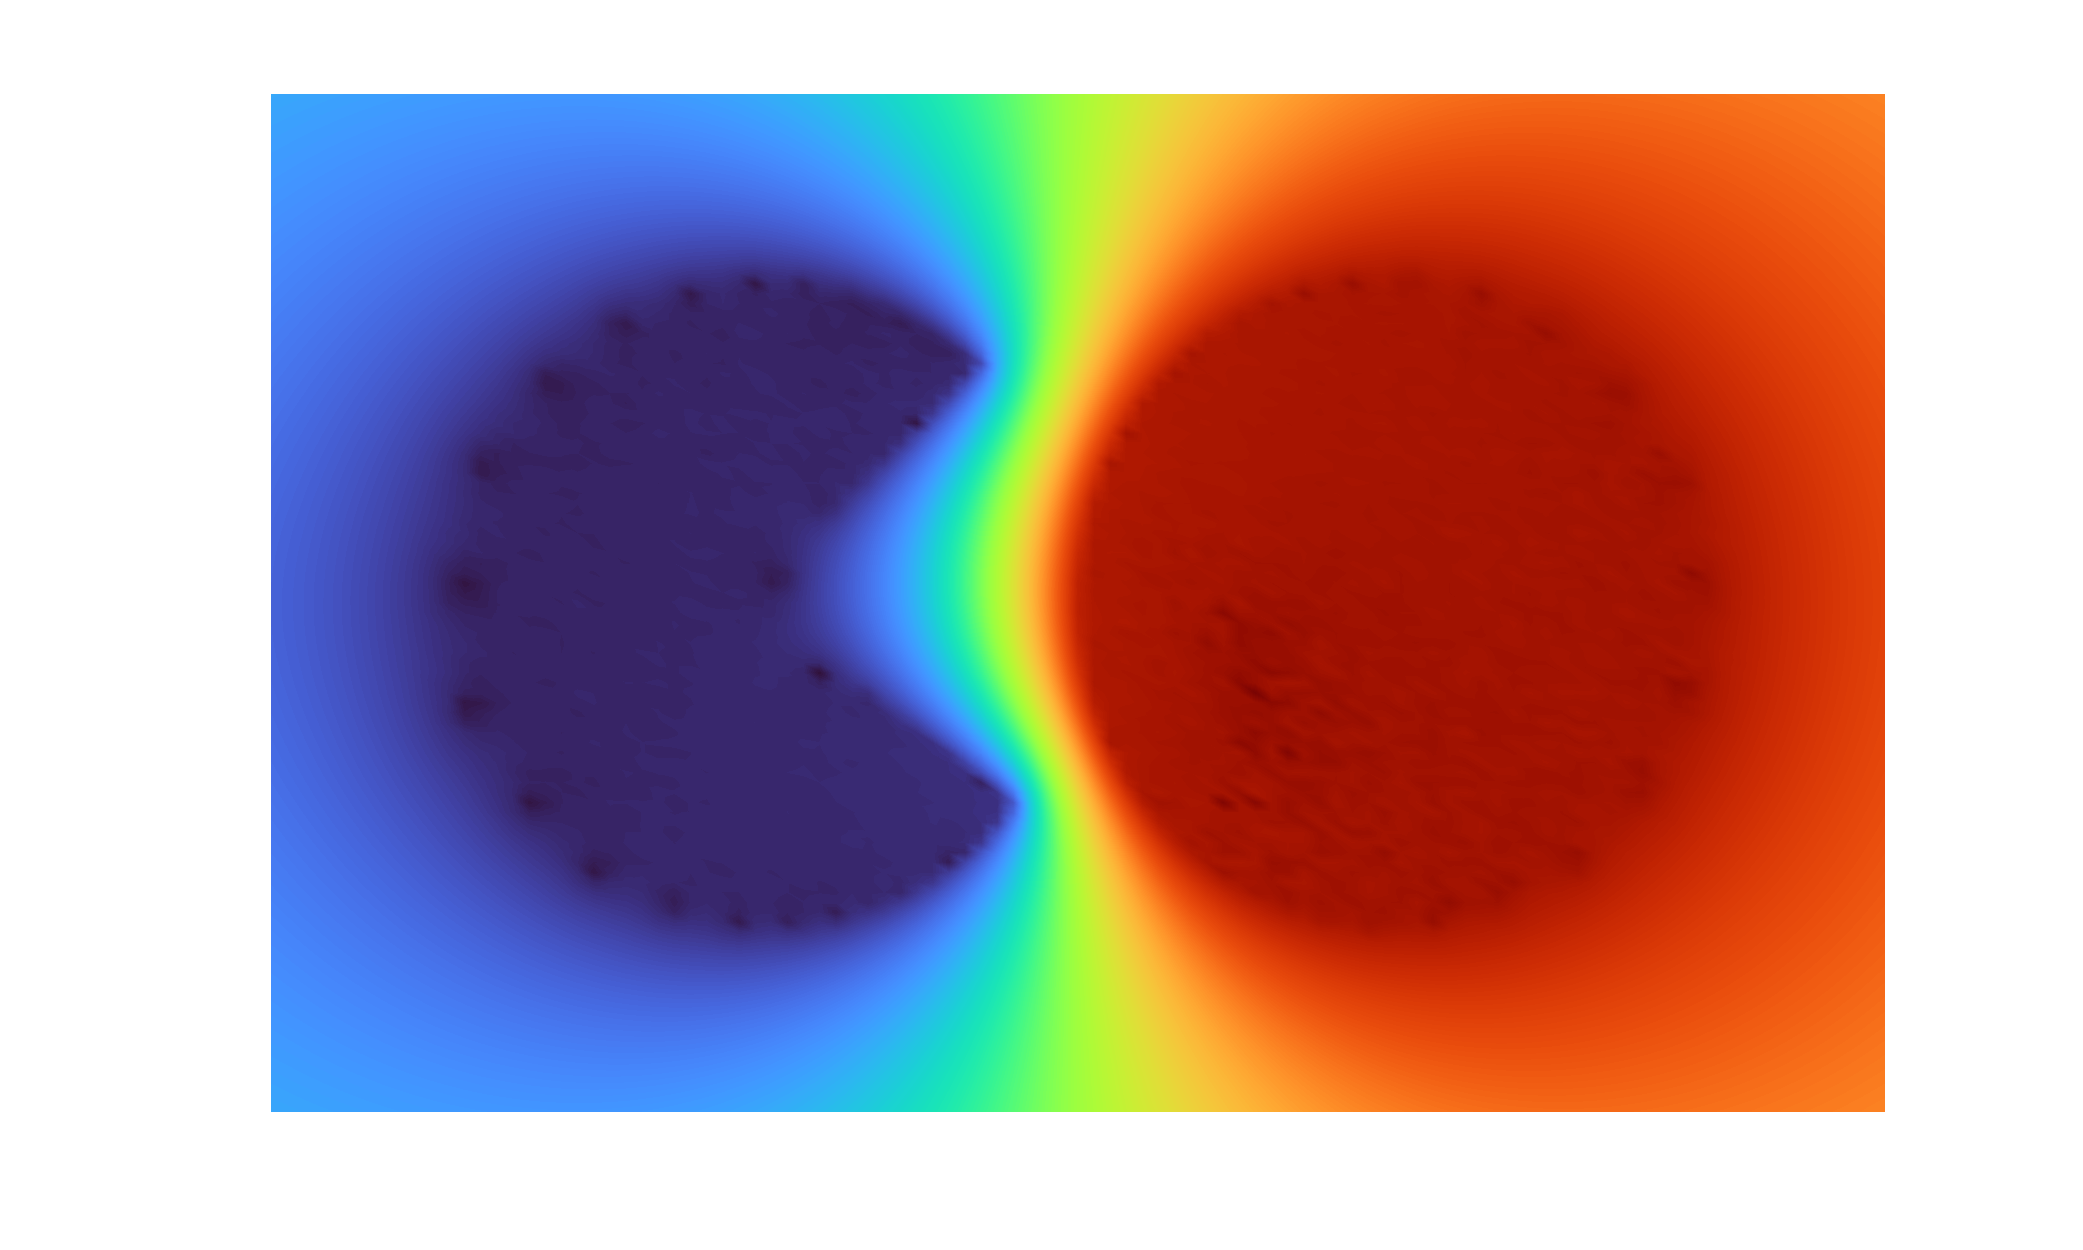
\includegraphics[width=.45\textwidth]{figures/art/pm2_2D}\\
Artistic views of the third Zoloratev problem applied to \\ the two symmetric circles (left) and Pac Man (left) topologies.
\end{center}


\section{Introduction and contributions}
\label{sec:intro}

\paragraph{About rational approximation.}

Approximation theory is a classic,  well-established field of mathematics, split into a wide variety of sub-fields, out of which we are particularly interested in approximation by rational functions. This has a multitude of applications in areas of applied sciences. Some examples include computational fluid dynamics, solution and control of partial differential equations, data compression, electronic structure computation, systems and control theory (model order reduction of dynamical systems).  For more details of the many aspects of approximation theory, we refer the reader to the classical books in \cite{Da75,Po81}, and to the more recent books \cite{Tr13,Is18} that also put emphasis on practical issues such as software implementation of the methods and applications, i.e., on data analysis for the latter.

Since rational functions are ratios of two polynomials, they have proven to be more versatile in approximating complex functions than simple polynomials. Furthermore, rational functions are extensively used in signal processing, systems, and control theory since the input-output behavior of linear dynamical systems is described in the frequency domain by the so-called transfer function (which is a rational function). Finally, the location of the poles of transfer functions determines important system properties such as asymptotic stability, transient behavior, damping, and harmonics.

\paragraph{Preliminaries on the Zoloratev 3rd and 4th problems and the data-driven framework.}

We are concerned with rational approximation, i.e.,  approximation of any type of functions, by means of rational ones. Here, we consider sign and ratio Zolotarev functions whose solution is intertwined. More precisely, the original function to be approximated falls into the category of a special sign function, defined on the complex domain, i.e., one that is defined on a reunion of two domains $E$ and $F$, for which the value is constant on each, e.g., equal to $\pm 1$ (hence the name Zolotarev sign problem, Z4, \cref{pb:z4}). To find the solution to the Zolotarev ratio function, one may appropriately transform the previously obtained solution. What is obtained is a function that is large on one domain ($F$), and small on the other ($E$), and thus, their ratio is minimized (hence the name Zolotarev ratio problem, Z3, \cref{pb:z3}). 

Moreover, the methods we use to solve Zolotarev sign problems do not require access to the exact closed-form of the original function, but only to evaluations of it on a particular domain. Hence, these methods are \emph{data-driven}.

In this work, we apply two established data-driven rational approximation methods: the Loewner Framework (LF) introduced in \cite{ajm07}, and the Adaptive Antoulas-Anderson (AAA) algorithm introduced in \cite{nst18}, and further developed in \cite{nakatsukasa2020algorithm,trefethen2024computation}. 
The methods mentioned above have some things in common: they both compute approximants in the form of rational functions, they exclusively use measurements of the original function (and not the function itself), and they involve, in one way or another, Loewner matrices.

\subsection{Contributions}
We summarize below the main contributions of this paper, which were confirmed through a series of comprehensive numerical experiments:
\begin{itemize}
    \item[(i)] we show that the LF solves Zolotarev problems by compressing the (many) number of  interpolation points. This approach does not need neither any iterations nor user intervention, and yields solutions quite close to the optimal ones in a very low computational time. Consequently, the LF constitutes a valid alternative for addressing these problems;
    \item[(ii)] we show that, in some specific cases (notably the symmetric two circles one), LF recovers the structure of the optimal solution as well as its symmetry property (e.g., the distribution of eigenvalues and zeros, the alternance of polynomials coefficients, realness, etc.), whereas the other methods tend to add spurious and oddly distributed poles and zeros, and non-trivial artifacts that can't be easily explained. In addition, thanks to an extensive numerical experimentation, we demonstrate the numerical robustness in the results obtained with LF compared to AAA\footnote{Up to the author's knowledge, this property has not been highlighted in previous works.};%Such a feature is crucial for discovering the properties of the topology when only data values are available
    \item[(iii)] we conduct an extensive numerical study\footnote{Results can be re-computed using the code available at \url{https://github.com/cpoussot/zolotarev}.} and comparison of the performance of different methods\footnote{The AAA algorithm uses the code available at \url{https://github.com/chebfun/chebfun}.} w.r.t. to computing time, accuracy of fit and interpretability, for approximating several sign functions defined on various domains showing, among others, the computational advantage of LF.
\end{itemize}

\subsection{Paper structure}
This paper is organized as follows: after the introduction in \cref{sec:intro}, in \cref{sec:zolo}, the Zolotarev sign and ratio problems are presented. Then, \cref{sec:ratapp} describes the main rational approximation tools to be used later on, e.g., the Loewner Framework in \cref{sec:Loew} and the AAA algorithm in \cref{sec:AAA}. We keep the exposition brief, since both are established methods, and we refer to the original manuscripts for details. Then, in \cref{sec:1a}, the special symmetric two circles topology is treated (i.e., for which the $E$ and $F$ domains are two symmetric circles). For this configuration, a detailed analysis of the results obtained by LF and AAA is discussed. The latter is not restricted to the approximation metric but also includes the values of the obtained numerators and denominators polynomials, poles and zeros, etc. (more details are available in \cref{app:1a}). Then,  in \cref{sec:num}, we conduct an exhaustive numerical experiments for various test cases, including the ones in \cite{trefethen2024computation} (more details are available in \cref{app:all}). Finally, applications of Zolotarev problems are presented in  \cref{app:applications}. Conclusions are discussed in \cref{sec:conclusion}.

%%%%%%%%%%%%%%%%%%%%%%%%%%%%%%%%%%%%%%%
\section{The Zolotarev problems}\label{sec:zolo}

In \cite{trefethen2024computation}, a detailed historical account is presented, which is summarized next. Additionally, we refer the reader to the review paper \cite{nakatsukasa2016computing} for further considerations.

\subsection{Reminder and general procedure}

For integers $m,n\ge 0$, let $R_{m,n}$ (or simply $R_n$ if $m=n$) be the set of rational functions with numerator of degree $m$ and denominator of degree $n$, which means that any rational function $r\in R_{m,n}$ can be written as $p(\varIC)/q(\varIC)$ for some polynomials $p(\varIC)$ and $q(\varIC)$ of degrees at most $m$ and $n$, respectively. The problem  studied here is to find $r_{m,n}^*\in R_{m,n}$ such that
\begin{equation}
r_{m,n}^* := \arg \min_{r\in R_{m,n}} {\max_{\varIC\in E} |r(\varIC)| \over \min_{\varIC\in F} |r(\varIC)|}.
\label{unscaled}
\end{equation}
%Since multiplying $r$ by a constant does not change the ratio, we may normalize the problem by fixing
Through normalization, i.e., assuming that $\min_{\varIC\in F} |r(\varIC)| = 1$, we end up with the problem of minimizing $|r(\varIC)|$ solely over set $E$. This is known in the literature as the third Zolotarev problem, or sometimes, also the {\em Zolotarev ratio problem}.

\begin{problem}[Zolotarev ratio problem - Z3]\label{pb:z3}
Find $r_{m,n}^*\in R_{m,n}$, satisfying condition $\min_{\varIC\in F} |r_{m,n}^*(\varIC)| = 1$, and that attains the minimum (where $\|\cdot\|_E^{}$ denotes the supremum norm over $E$)
\begin{equation}
\sigma_n = \min_{r \in R_{m,n}} \|r\|_E^{}.
\label{Z3}
\end{equation}
\end{problem}

As mentioned in \cite{trefethen2024computation}, it is known that a solution $r_{m,n}^*$ to (\ref{Z3}) exists, though it need
not be unique, and that $\sigma_n$ satisfies $0 < \sigma_n \le 1$.

Then, the {\em sign function} relative to $E$ and $F$ is of relevance in what follows, and is defined as follows:
\begin{equation}
\signEF(\varIC) =
\begin{cases}
-1 & \varIC\in E, \\ +1 & \varIC\in F.
\end{cases}
\end{equation}
It is to be noted that for $z\in\IC\backslash \{E\cup F\}$, $\signEF(\varIC)$ remains undefined.

Next, we introduce the problem of rational minimax approximation of $\signEF$ over $E$ and $F$, or problem Z4: 

\begin{problem}[Zolotarev sign problem - Z4]\label{pb:z4}
Find $\hat r_{m,n}\in R_{m,n}$ that attains the minimum (where $\|\cdot\|_{E\cup F}$ denotes the supremum norm over $E\cup F$)
\begin{equation}
\tau_n = \min_{r\in R_{m,n}} \|r-\signEF\|_{E\cup F}^{}.
\label{Z4}
\end{equation}
\end{problem}

As mentioned in \cite{trefethen2024computation}, the proof showing that the problems Z3 and Z4 are equivalent in the case for which $E$ and $F$ are real intervals is due to the work of \cite{akhiezer1990elements}. Then, in \cite{istace1995third}, it was shown that the equivalence generalizes to the complex case.  We reproduce (with appropriate notation changes) in what follows their theorem.

\begin{theorem}
\label{thm1}
Every solution $r_{m,n}^*$ of Problem Z3 is related to a solution 
$\hat r_{m,n}$ of Problem Z4 by
\vspace{-2mm}
\begin{equation}
\hat r_{m,n} (\varIC) = {1-\sigma_n\over 1+\sigma_n} \,{r_{m,n}^*(\varIC) - \sqrt{\sigma_n}
\over r_{m,n}^*(\varIC) + \sqrt{\sigma_n}}, \quad
r_{m,n}^*(\varIC) = \sqrt{\sigma_n} \,
{(1-\sigma_n)/(1+\sigma_n) + \hat r_{m,n}(\varIC) \over
(1-\sigma_n)/(1+\sigma_n) - \hat r_{m,n}(\varIC)}.
\label{relation}
\end{equation}
The minimal values of the two problems satisfy
\vspace{-2mm}
\begin{equation}
\tau_n = {2\sqrt\sigma_n\over 1 + \sigma_n}, \quad
\sigma_n = \left({\tau_n\over 1 + \sqrt{1-\tau_n^2}\kern .7pt} \right)^2,
\label{minvals}
\end{equation}
and the set of extremal points $M = \{z\in E\cup F, ~|\hat r_{m,n}(\varIC) - \signEF(\varIC)| = \tau_n\}$ is the union of  $M_1 = \{z\in E, ~|r_{m,n}^*(\varIC)| = \sigma_n\}$ and $M_2 = \{z\in F, ~|r_{m,n}^*(\varIC)| = 1\}$.
\end{theorem}

% \charles{USEFULL?
% In the standard case for which $\tau_n, \sigma_n\ll 1$, \eqref{relation} and \eqref{minvals}, it follows that the approximate values below hold true:
% \begin{equation}
% \hat r_n^{} (\varIC) \approx {r_n^*(\varIC) - \sqrt{\sigma_n}
% \over r_n^*(\varIC) + \sqrt{\sigma_n}}, \quad
% r_n^*(\varIC) \approx {\tau_n\over 2} \,
% {1+ \hat r_n^{}(\varIC) \over 1- \hat r_n^{}(\varIC)}
% \label{relation2}
% \end{equation}
% and also that $\tau_n \approx 2\sqrt\sigma_n$, $\sigma_n \approx {\tau_n^2\over 4}$.
% }

\subsection{Approach paved in  \cite{trefethen2024computation} and discussions}

The proposed algorithms for solving \cref{pb:z3} (Z3) actually consist of solving \cref{pb:z4} (Z4) first, and then transforming from $\hat r_{m,n}$ and $\tau_n$ to $r_{m,n}^*$ and $\sigma_n$. Following \cref{thm1}, the authors of \cite{trefethen2024computation} approach Problem Z3 in the following two-step procedure: (i) solve Problem Z4 using a rational approximation method; then (ii) convert to a solution of Problem Z3 using \cref{relation} and \cref{minvals}.

The main challenge of the algorithm proposed in \cite{trefethen2024computation} is given by step (i), i.e., the computation of the degrees $(m,n)$ rational best approximation $\hat r_{m,n}$ to the sign function $\signEF$ defined by the sets $E$ and $F$.  In \cite{trefethen2024computation}, the proposed procedure is to find $\hat r_{m,n}$ by means of the AAA approximation technique.  However, this has proven quite challenging. The first difficulty reported in \cite{trefethen2024computation} is that AAA encounters particular challenges when applied to sign functions. The second is the importance of having not just good rational approximations but nearly optimal ones, requiring the use of the AAA-sign and AAA-Lawson algorithm \cite{nakatsukasa2020algorithm}, which had a known problem of non-convergence in certain cases. These difficulties and their proposed solutions are discussed in \cite[\S 3.1 and \S 3.2]{trefethen2024computation}. Basically, the Lawson iteration "drives" the standard AAA approximant close to the optimal approximation value by performing several least squares steps involving  the weights. Although seemingly effective, this approach has proven to be quite costly, mostly in terms of running time, but also in terms of the structure of the resulting polynomials, as will become evident in the next sections. This is particularly relevant when choosing a high degree $(m,n)$ for the approximant. In addition, as highlighted in the coming sections, AAA (and its extensions) results vary according to the computer platform used.

%\subsection{Applications of the Z3 and Z4 problems}
%
%\paragraph{Zolotarev ration problems (Z3).}
%
%\paragraph{Zolotarev sign problems (Z4).}


%%%%%%%%%%%%%%%%%%%%%%%%%%%%%%%%%%%%%%%
\section{The main approximation methods}\label{sec:ratapp}



\subsection{The Loewner framework}\label{sec:Loew}

The Loewner Framework (LF) is a data-driven model identification, approximation, and reduction tool introduced in \cite{ajm07}. It provides a simple solution through rational approximation by means of interpolation. For more details, we refer the reader to the extensive tutorial/handbook papers in \cite{morKarGA19a,morGosPA22,ali17}, and to the papers \cite{morIonA14,AGPV:2025,morAntGI16,morKarGGetal25} that address extensions of the LF to some special classes of parametric, nonlinear or hybrid dynamical systems, and to  the recent book of interpolation and model reduction \cite[chapter 4]{abg_book}. 

%Recently, an extension of LF for approximating the absolute value function was presented in \cite{LoewAbsVal}.

%For more details, we refer the reader to the extensive tutorial paper \cite{ali17}, the Ph.D. dissertation in \cite{Io13} that addresses connections of the LF to Lagrange rational interpolation, the Ph.D. dissertations in \cite{Go17,morKar23} that address extensions of the LF to some special classes of nonlinear and hybrid dynamical systems, the tutorial/handbooks papers in \cite{morKarGA19a,morGosPA22}, and to chapter 4 in the recent book \cite{abg_book}.


Given $N>0$ distinct sampling points $\cT = \{\tau_1, \tau_2, \ldots,\tau_N\}$ together with $N$ function evaluations at these points denoted with $\{f_1, f_2, \ldots,f_N\}$, let $\mathfrak{D} = \{(\tau_\ell; \  f_\ell) \vert \ell =1,\cdots,N\}$ to be the problem data. Assume that $N=k+q$, where $k$ and $q$ are positive integers. The given data $\mathfrak{D}$ is first partitioned into the following two disjoint subsets,
\vspace{-2mm}
\begin{equation}\label{data_Loew}
\mathfrak{D} = \mathfrak{L} \cup \mathfrak{R}, \ \text{where} \ \begin{cases} {\text{right data}}: \mathfrak{R} = \{(\lambda_i; \  w_i) \vert i=1,\cdots,q
\}, \\
 {\text{left data}}: \ \ \mathfrak{L} =
\{(\mu_j; \ v_j) \vert j=1,\cdots,k\}. \end{cases}
\end{equation} 
%(for simplicity all points are assumed distinct).
The elements of the subsets $\mathfrak{L}$ and $\mathfrak{R}$ are as follows (for $1 \leq i \leq q$ and $1 \leq j \leq k$):
\begin{enumerate}
    \item  $\lambda_i$, $\mu_j$ $\in\IC$ are the right, and, respectively, left \emph{sample/interpolation points}.
	\item  $w_i$, $v_j$ $\in\IC$ are the right, and, respectively, left \emph{sample values}.
\end{enumerate}
The problem can be formulated as follows: find a rational function $\rloe(\varIC)$ of order $r \ll k$, such that the following interpolation conditions are (approximately) fulfilled:
\begin{equation} \label{interp_cond}
\rloe(\lambda_i)=w_i,~~~\rloe(\mu_j)=v_j.
\end{equation}
%The first step is to partition the data in two disjoint categories, i.e the \textit{right data}
%\vspace*{-2mm}
%\begin{equation}
%\Lambda=\rm{diag}(\lambda_1,\lambda_2,\ldots,\lambda_k)\in\IC^{k\times k},~ \bW=[\bw_1~~\bw_2~~\cdots~~\bw_k]\in\IC^{1\times k}.
%\end{equation}
%and the the \textit{left data}
%\vspace*{-2mm}
%\begin{equation}
%\bM=\rm{diag}(\mu_1,\mu_2,\ldots,\mu_k)\in\IC^{k\times k},~
%\bV=\left[\!\begin{array}{cccc} \bv_1^*&\bv_2^*&\ldots&\bv_q^*
%\end{array}\!\right]^*\in\IC^{k \times 1}. 
%\end{equation}

%\charles{NOT SURE IS NEEDED
%\begin{remark}
%Note that in a typical data-driven MOR setup, it is considered that the sample values  $w_i$, $v_j$ $\in\IC$ represent evaluations of the function $H(\varIC)$. More precisely, one would assume that $H(\lambda_i)  =w_i$ and $H(\mu_j)  =v_j$ for all $1 \leq i,j \leq k$.
%\end{remark}
%}

The next step is to arrange data (\ref{data_Loew}) into matrix format. The \textbf{Loewner matrix} $\IL \in\IC^{k\times q}$ and the \textbf{shifted Loewner matrix} $\sIL \in\IC^{k\times q}$ are defined as
\begin{equation} \label{Loew_mat}
\IL=\left[\begin{array}{ccc}
\frac{v_1-w_1}{\mu_1-\lambda_1} & \cdots &
\frac{v_1-w_q}{\mu_1-\lambda_q} \\
\vdots & \ddots & \vdots \\
\frac{v_k-w_1}{\mu_k-\lambda_1} & \cdots &
\frac{v_k-w_q}{\mu_k-\lambda_q} \\
\end{array}\right], \ \ 
\sIL=\left[\begin{array}{ccc}
\frac{\mu_1v_1-w_1\lambda_1}{\mu_1-\lambda_1} & \cdots &
\frac{\mu_1v_1-w_q \lambda_q}{\mu_1-\lambda_q} \\
\vdots & \ddots & \vdots \\
\frac{\mu_kv_k-w_1 \lambda_1}{\mu_k-\lambda_1} & \cdots &
\frac{\mu_kv_k-w_q\lambda_q}{\mu_k-\lambda_q} \\
\end{array}\right],
\end{equation}
while the data vectors $\bV\in \IR^k, \bW^\top \in \IR^q$ are introduced as
\begin{equation} \label{VW_vec}
\bV=\left[\!\begin{array}{cccc} v_1 \  \ v_2 \  \ \ldots \  \ v_k \end{array}\!\right]^\top \in \IC^k, \ \ \ \bW=[w_1~~w_2~~\cdots~~w_q] \in \IC^q.
\end{equation}

\begin{lemma}
	If $k=q$ the matrix pencil $(\sIL,\,\IL)$ is regular, then one can directly compute the  interpolation function as below:
	\begin{equation}
	\rloe(\varIC)=\bW(\sIL-\varIC \IL)^{-1}\bV.
	\end{equation}
   % \charles{NOT USEFULL? together with the Loewner model composed of $\bE=-\IL,~~ \bA=-\sIL,~~ \bB=\bV,~~ \bC=\bW$.}
\end{lemma}

In applications (see, e.g., \cite{morGosPA22}), the pencil $(\sIL,\,\IL)$ is often singular. In these cases, one needs to perform an SVD of the Loewner pencil, constructed from the row- and column-wise concatenation of matrices $\IL$ and $\sIL$. By choosing a truncation value $r$, we can write the truncated SVDs as follows (with $\bX_r = \bX_r^{(1)} \in \IC^{k \times r}$, $\bY_r = \bY_r^{(2)} \in \IC^{q \times r}$)
\begin{equation}\label{eq:loew-rank}
%\begin{cases} 
\begin{bmatrix} \IL & \sIL \end{bmatrix} \approx \bX_r^{(1)} \bS_r^{(1)} {\bY_r^{(1)}}^* ,~
\begin{bmatrix} \IL \\ \sIL \end{bmatrix}  \approx \bX_r^{(2)} \bS_r^{(2)} {\bY_r^{(2)}}^*. %\end{cases}
\end{equation}	
\begin{lemma}			
	The rational function corresponding to the reduced-order Loewner model is derived as:
	%\begin{align}\label{loew_fct}
	%\begin{array}{rcl}
    \begin{align*}
	\rloe(\varIC) = \hat{\bC}_{\mathrm{Loew}} (\varIC \hat{\bE}_{\mathrm{Loew}}-\hat{\bA}_{\mathrm{Loew}})^{-1} \hat{\bB}_{\mathrm{Loew}} 
    =  \bW \bY_r \Big{(} \bX_r^* (\sIL- \varIC \IL) \bY_r \Big{)}^{-1} \bX_r^* \bV,
    %\end{array}
	\end{align*}
    where the system matrices corresponding to a reduced Loewner model are:
    	\begin{equation} \label{Loew_red_mat}
	\hat{\bE}_{\mathrm{Loew}} = -\bX_r^*\IL \bY_r, \ \  \hat{\bA}_{\mathrm{Loew}} = -\bX_r^*\sIL \bY_r, \ \
	\hat{\bB}_{\mathrm{Loew}} = \bX_r^*\bV, \ \  \hat{\bC}_{\mathrm{Loew}} = \bW \bY_r.
	\end{equation}
\end{lemma}


\subsection{The AAA algorithm (and variants)}\label{sec:AAA}


The AAA (Adaptive Antoulas-Anderson) algorithm proposed in \cite{nst18} represents an adaptive extension of the method originally introduced by A.C. Antoulas and B.D.O. Anderson in \cite{aa86}. The AAA algorithm is a rational approximation data-based method that makes use of the barycentric form of rational functions and uses an iteration to add more interpolation points (in a greedy fashion) until a certain level of approximation is attained. As exposed in \cref{sec:Loew}, it only requires as input evaluations of the function on a set of points denoted with $\cT$. We refer to \cite{AAAreview} for a recent review paper on applications of AAA.

%\subsubsection{Original version}\label{sec:aaa_original}

Consider $N>0$ distinct sampling points in the set $\cT = \{\tau_1, \tau_2, \ldots,\tau_N\}$ together with $N$ function evaluations at these points, denoted with $\{f_1, f_2, \ldots,f_N\}$.
The AAA algorithm is based on an iteration. 
Let the order of the rational approximant $\raaa(\varIC)$ that is constructed through the algorithm in \cite{nst18} at step $\ell \geq 1$ be $(\ell,\ell)$ (degree of numerator and denominator), which is written in the following barycentric format: 
\begin{equation}\label{AAA_approx}
\raaa(\varIC) = \frac{ \sum_{k=0}^\ell \frac{ \alpha_k w_k }{\varIC - \lambda_k }}{ \sum_{k=0}^\ell \frac{\alpha_k }{\varIC- \lambda_k}},
\end{equation}
where $\{\lambda_0,\ldots,\lambda_\ell\}$ are the interpolation points (selected from the set $\cT$), $\{w_0,\ldots,w_\ell\}$ are the corresponding function evaluations, and $\{\alpha_0,\ldots,\alpha_\ell\}$ are the weights. The method enforces interpolation at the $\ell$ points $\{\lambda_0,\ldots,\lambda_\ell\}$, i.e. $\raaa(\lambda_k) = w_k = F(\lambda_k), \, \forall \, 0 \leqslant k \leqslant \ell$. Then, at each step, one needs to determine suitable weights $\alpha_0,\alpha_2,\ldots,\alpha_\ell$ by formulating an approximation problem. Instead of solving the more general problem above (which is nonlinear in variables $\alpha_1, \alpha_2, \ldots, \alpha_\ell$), one solves a relaxed problem by means of linearization. This procedure leads to a least squares minimization problem that involves a (rectangular) Loewner matrix of dimension $(N-\ell) \times \ell$. The solution relies on computing the SVD of the latter, and selecting the weights as the entries of the (normalized) last right singular vector.
At the end of the iteration, the rational approximant is of order $(r,r)$; one can also explicitly write the AAA function as $\raaa(\varIC) = \hat{\bC}_{\mathrm{AAA}} (\varIC \hat{\bE}_{\mathrm{AAA}}-\hat{\bA}_{\mathrm{AAA}})^{-1} \hat{\bB}_{\mathrm{AAA}}$,
where the matrices are of dimension $r=\ell+1$, given explicitly in terms of the selected support points  $\{\lambda_0,\ldots,\lambda_r\}$, the function evaluations $\{w_0,\ldots,w_r\}$ and the weights $\{\alpha_0,\ldots,\alpha_r\}$. Note that for the numerical examples presented in what follows, we will be using the AAA implementation available in the \chebfun~ tool \cite{chebfun}\footnote{Also available at \url{https://github.com/chebfun/chebfun}.}.

%\subsubsection{Minimax algorithms and Lawson step extensions}\label{sec:minimax}


% The problem that is addressed in the contribution \cite{fntb18} is to approximate functions $f \in \cC([a,b])$ using type $(m,n)$ rational approximations with real coefficients from the set $\cR_{m,n}$.


% Given the function $f$ and integers $m,n$, the problem is formulated as follows: find $r \in \cR_{m,n}$ so that the infinity norm $\Vert f - r \Vert_\infty = \max_{x \in [a,b]} \vert f(\varIC) - r(\varIC) \vert$ is minimized.
% It is known that such a minimizer exists and is unique (Chapter 24 in  \cite{Tr13}).

% Denote with $\overline{r} \in \cR_{m,n}$ the best (minimax) approximation of the function $f$ (the solution to the above problem). It follows that there exists a sequence of ordered nodes where the function $f-r^*$ takes its global extreme value over the interval $[a,b]$ (with alternating signs). This sequence is denoted with $(x_0,x_1,\ldots,x_{m+n+1})$ with  $a \leqslant x_0 < x_1 < \cdots < x_{m+n+1} \leqslant b$, hence
% \begin{equation}
% f(x_k)-\overline{r}(x_k) = (-1)^{k+1} \Vert f - \overline{r} \Vert_{\infty}, \ \ \ k \in \{0,1,\ldots,m+n+1\}.
% \end{equation}

Computing rational minimax approximations is a challenging task, especially when there are singularities on or near the interval of approximation. In the recent contribution \cite{fntb18}, the authors propose different combinations of robust algorithms that are based on rational barycentric representations. One key feature is that the support points are chosen adaptively as the approximant is computed. The \chebfun~ minimax implementation is available in  \cite{chebfun}. The  AAA-Lawson algorithm in \cite{nakatsukasa2020algorithm} uses an iteratively re-weighted least-squares method followed by a classical Remez algorithm to enforce  quadratic convergence. Minimax approximants can be recognized by their equioscillatory error curves in real cases and nearly circular error curves in complex problems.

%In \cite{trefethen2024computation}, the general idea is to improve rational approximations from near-best (AAA) to best (minimax) through the AAA-Lawson iteration.  As described in Section 3 of \cite{nakatsukasa2020algorithm}, this is a nonlinear variant of iteratively reweighted least-squares, which often converges to minimax approximations.  The centerpiece of the Lawson iteration is an adjustment of the weights in a least-squares problem (linear) according to the errors at the same points in the current rational approximation (nonlinear). 

In the recent note \cite{trefethen2024computation}, the authors present an algorithm based on AAA-Lawson approximation~\cite{nakatsukasa2020algorithm}, enhanced by various modifications that make it suitable for dealing with functions of the flavor of $f(\varIC) = \hbox{sign}(\varIC)$ and for ensuring convergence of the Lawson phase. This variant/improvement of the standard AAA algorithm in \cite{nst18} is meant as a reliable tool for numerical computations of solutions for the third and fourth Zolotarev problems, i.e., classical problems in approximation theory.

%Hence, these developments presented in \cite{trefethen2024computation} are deemed a "breakthrough", since, we quote, "a reliable method for computing these functions has not been available before". 

An attentive reader may realize that in \cite{trefethen2024computation}, these developments are deemed a "breakthrough" since "a reliable method for computing these functions has not been available before". However, the LF is known since 1986 in its one-sided version \cite{aa86} and since 2007 in its two-sided version \cite{ajm07} (the latter was used in this work).

%However, one point we would like to make in this work is that the LF has been around for almost two decades, and can be used as a reliable and direct surrogate to methods based on iteration and optimization steps, such as AAA-Lawson in \cite{trefethen2024computation}. 

%%%%%%%%%%%%%%%%%%%%%%%%%%%%%%%%%%%%%%%
\section{The two symmetric circles case}
\label{sec:1a}

\subsection{Experimental setup and results} 

We start the numerical exposition with a rather simplified configuration, namely the two symmetric circles case. This configuration is also denoted \texttt{'1a'} in \cite{trefethen2024computation}. For this topology, the true optimal rational approximation solution for the Zolotarev problem Z4 is explicitly known. Let us consider two circles $E$ ($-1$) and $F$ ($+1$) symmetric (with respect to the imaginary axis), centered along the horizontal axis, with radius $\rho$ and centered at $\pm \alpha$. In this case, the optimal rational $r$-th order approximant $r_r^*(\varIC)$ derived in \cite{starke1992near} is given by:
\begin{equation}
r_r^*(\varIC) = \left(\dfrac{\varIC-\sqrt{\alpha^2-\rho^2}}{\varIC+\sqrt{\alpha^2-\rho^2}}\right)^r
\text{ and }
\sigma_r = \left(\dfrac{1-\sqrt{\alpha^2-\rho^2}}{1+\sqrt{\alpha^2-\rho^2}}\right)^r.
\label{eq:case_1a_opt}
\end{equation}

The case considered in what follows corresponds to the one in \cite[Figure 1(a)]{trefethen2024computation},  for which $\rho = 1/2$ and $\alpha = 1$ (see also \cref{fig:intro:1a} and \cref{fig:intro:1a_1e14}). To compare the rational approximation obtained for problem Z4 using either LF or AAA, the following two scenario will be used (see also \cref{sec:num} for LF code description):
\begin{itemize}
\item[S1] (i) the LF, (ii) the AAA, (iii) the AAA-sign(damping) and (iv) the AAA-sign(damping)-Lawson (with 200 iterations)\footnote{The AAA results are obtained with optional arguments  \texttt{'sign',0,'lawson',0}, \texttt{'sign',1,'damping',.95} and \texttt{'sign',1,'damping',.95,'lawson',200}, using the AAA code in \chebfun.}. 
\item[S2] (i) the LF, (ii) the AAA-Lawson (with 200 iterations) and (iii) the AAA-Lawson (with 1000 iterations)\footnote{The AAA-Lawson is obtained with optional arguments  \texttt{'sign',1,'damping',.95,'lawson',200} and \texttt{'sign',1,'damping',.95,'lawson',1000}, using the AAA code in \chebfun.}. 
\end{itemize}

\def\nLocal{4} 
\subsection{Structure analysis of the rational solutions}

We begin with a simple approximation with $r=\nLocal$. The \cref{fig:intro:1a} shows the topology, approximation and poles/zeros distributions for the scenario S1. More specifically,  we display the rational approximation for Z3 with contours, and both the poles and the zeros for Z3 and Z4. Each frame illustrates the rational approximation reached by each method.  Comparing solely the approximation metric $\sigma_\nLocal$ (in each frame titles), this figure shows that every methods but AAA (with no option) is able to achieve a good approximation. In addition, it also clearly emphasizes the superiority of AAA combined with sign and Lawson iterations, both  being very close to the optimal one given in  \cref{eq:case_1a_opt}.

\begin{figure}[ht!]
    \centering
    \includegraphics[width=.75\textwidth]{figures/all/cas_1a_r\nLocal.pdf}
    \caption{Case \texttt{'1a'}, with $r=\nLocal$: different approximation methods: LF (top left), AAA (top right), AAA with damping (bottom left), and AAA-Lawson with damping and  200 iterations (bottom right). Each frame shows: the Zolotarev rational functions of degree $r$ for Z3 ($\bh_3$) and Z4 ($\bh_4$) defined by connected sets $E$ (on the left) and $F$ (on the right); the Z3 function approximate contours levels $\log_{10} |\bh_3(\varIC)|= 0,-1,-2,\cdots,-30$ between the two domains; yellow circles and cyan blue dots respectively mark zeros and poles of the sign function $\bh_4$; blue and red dots respectively denote the zeros and poles of $\bh_3$. The minimum values $\sigma_r$ and computation time are given in the title, as well as the options of each AAA method. The number of singularities targeted (and obtained).}
    \label{fig:intro:1a}
\end{figure}


Now, let us focus on the AAA parametrizations leading to a good approximation and consider scenario S2. In the table below, we report the coefficients of both numerator and denominator (both real and imaginary parts) of the rational approximation obtained with each different method, and compare to the optimal Z4 approximant of the same order, obtained with \cref{eq:case_1a_opt} ($r=\nLocal$)\footnote{The caption mentions \texttt{cpv MACA64 MR2023b} since these results have been obtained by C. Poussot-Vassal on a Mac OS with \texttt{MATLAB} 2023b. See \cref{app:1a} for other architectures.}. The maximum approximation errors $\sigma_\nLocal$ are displayed for all approximants. 
\input{data/cpv_MACA64_MR2023b/tables/1a_nd_r\nLocal}

The first comment for this case is that the optimal rational approximation \cref{eq:case_1a_opt} is attained with a real-valued function and a rational complexity of degree $(r-1,r)$. Therefore, for $r=\nLocal$, one notices that:
\begin{itemize}
    \item LF provides a solution with real-valued coefficients only (up to machine precision), while both AAA-sign-Lawson end up with non-negligible imaginary coefficients;
    \item by inspecting the numerator (first row), both AAA-Lawson suggest a non-null coefficient along with the $\varIC^\nLocal$ basis entry, resulting in a rational complexity of $R_{\nLocal,\nLocal}$ while the LF indicates a null term, leading to a complexity $R_{\fpeval{\nLocal-1},\nLocal}$ (as the optimal one);
    \item by inspecting the numerator along with the even basis entries $\varIC^0,\varIC^2,\dots$ and denominator of along with odd  basis entries $\varIC^1,\varIC^3,\dots$, it appears that the optimal have null coefficients. Again, only LF recovers this property (up to machine precision) while AAA shows high magnitude coefficients.
    \item by inspecting the $\sigma_\nLocal$ values for each method, AAA-Lawson provides a better approximant (i.e., with a lower $\sigma_\nLocal$) than LF (which is better than standard AAA); moreover, AAA-Lawson actually provides the near-optimal $\sigma_\nLocal$.
\end{itemize}
Choosing different order $r$, one may observe that the previous remarks still hold true\footnote{We refer to the \url{https://github.com/cpoussot/zolotarev} page for an in-depth analysis.} (see extensive report in \cref{app:1a}). Continuing the analysis, the following tables report the zeros and poles associated to the numerator and denominator for each rational approximation. 
\input{data/cpv_MACA64_MR2023b/tables/1a_zer_r\nLocal}
\input{data/cpv_MACA64_MR2023b/tables/1a_pol_r\nLocal}

These tables emphasize that both the poles and zeros obtained with AAA-Lawson are quite far from the optimal ones and contain a non-negligible real part, while the LF ones are very close. In addition, as the AAA rational approximation coefficients have large imaginary parts, poles and zeros do not come in complex conjugate form, while LF results in almost perfect closed form. Then, one pole comes with a very large magnitude, far from the domain of interest. Finally, as AAA constructs a rational approximation of the type $R_{\nLocal,\nLocal}$, an additional zero appears.

\subsection{Accuracy and computational effort}

Let now continue with approximation for varying rational degrees. First we compare the approximation features for significantly higher orders, using again scenario S1. In \cref{fig:intro:1a_1e14}, the approximation order $r$ has been selected such that the normalized singular values of the LF are below $10^{-14}$ (as suggested in \cref{eq:loew-rank}); then, the same objective is used for the three other methods.

\begin{figure}[ht!]
    \centering
    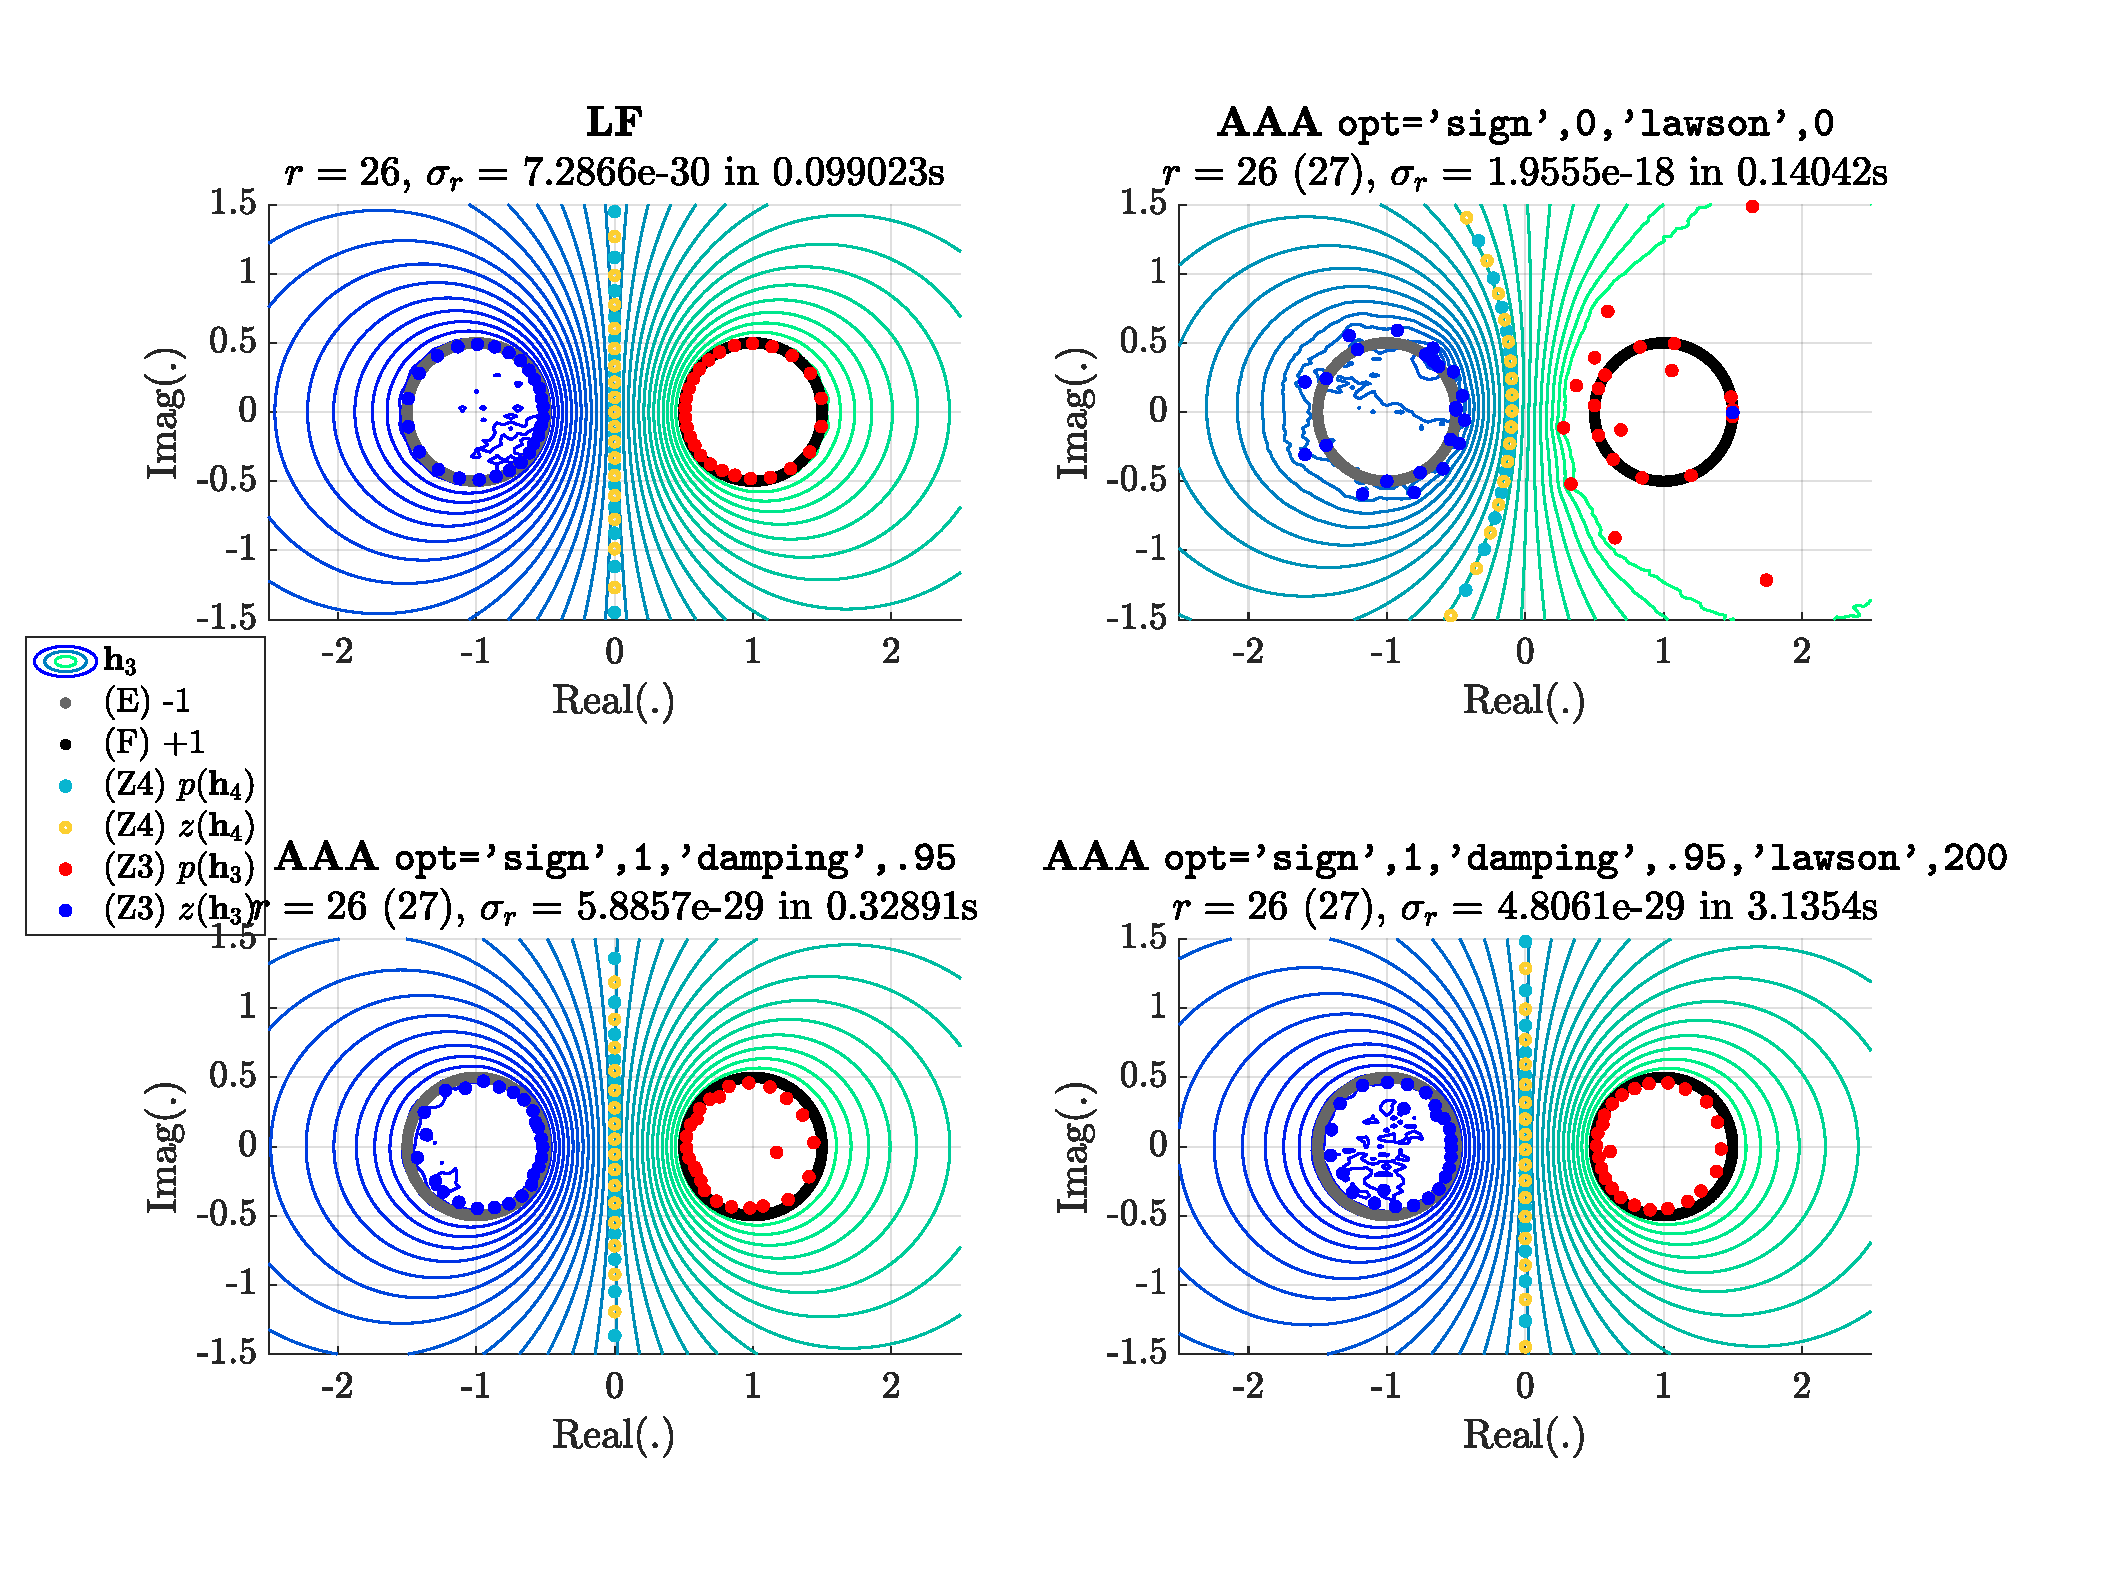
\includegraphics[width=.75\textwidth]{figures/all/cas_1a_r1e-14.pdf}
    \caption{Case \texttt{'1a'}, with $r=26$: same as \cref{fig:intro:1a}.}
    \label{fig:intro:1a_1e14}
\end{figure}

What is remarkable in \cref{fig:intro:1a_1e14}, for the LF case, is the neat distribution of the poles and zeros of both Z3 and Z4 problems along the $\pm 1$ circles and vertical axis, with a perfect symmetry. This feature is guaranteed by the almost perfect alternate null and non-null coefficients and the null (machine precision) imaginary part. All other methods provide a slightly irregular distribution with imaginary part in the monomial coefficients. Moreover, in this setup, the optimal $\sigma_r\approx1.8144\cdot 10^{-30}$ \cref{eq:case_1a_opt} while the LF reaches the best approximation with $\sigma_n\approx 7.2866\cdot 10^{-30}$, very close to the optimal one. Notice also that the computation time is much lower for the LF with respect to the AAA versions, and even more with respect to the AAA-Lawson. 

This computational time is indeed an important point from practical considerations. By now evaluating the Zolotarev ratio and computation time for different  rational approximation orders $r$, the \cref{fig:intro:1a_time} is obtained. One observes that the LF requires a constant computation time while the AAA variants are dependent on the approximation order $r$. Indeed, LF benefits from the fact that it is not iterative. 

\begin{remark}[Accelerating LF]
As the LF consists in (i) building the Loewner pencil \cref{Loew_mat}, (ii) computing two SVDs \cref{eq:loew-rank}, and then (iii) truncating / projecting accordingly \cref{Loew_red_mat}, in practice, steps (i) and (ii) may be computed once; then step (iii) must be computed for each truncation order. A direct consequence is the computational effort is limited to the first computation and the rest will be simply projections with a marginal cost. This procedure may not be applied to the AAA.
\end{remark}

Considering the accuracy, AAA-sign-Lawson generally provides a slightly better ratio number $\sigma_r$ for almost all $r$. However, it reaches a plateau for higher orders ($r>25$), which is anyway hard to distinguish with rounding numerical accuracy.

\begin{figure}[ht!]
    \centering
    
\includegraphics[width=.75\textwidth]{figures/time_accuracy/cas_1a_zol_time.pdf}
    \caption{Case \texttt{'1a'}: computation time and accuracy for different approximation settings.}
    \label{fig:intro:1a_time}
\end{figure}

\subsection{Numerical robustness} 

We push our investigation by evaluating the results of the LF and AAA algorithms over different computer architectures settings, using scenario S2. More specifically, the code named \texttt{report\_1a\_step1}\footnote{Available at \url{https://github.com/cpoussot/zolotarev}.} has been executed on \NARCH~ different computers, with different architecture or \texttt{MATLAB} version (or both). Results were stored and analyzed via \texttt{report\_1a\_step2}, and dispersion of the numerator and denominator coefficients computed in \texttt{report\_1a\_step3}. This procedure applied to the case $r=\nLocal$, led to \cref{fig:intro:numden}. It shows the distribution of the rational approximation coefficients (numerator and denominator) according to the running machine. 

\begin{figure}[ht!]
    \centering
    \includegraphics[width=.75\textwidth]{figures/1a/num_den_r\nLocal.pdf}
    \caption{Case \texttt{1a}, $r=\nLocal$, Z4. Numerators and denominators real and imaginary coefficients dispersion over the \NARCH~ different platforms. For each frame, the $x$-axis refers to the monomial basis $\varIC$ degree, and the $y$-axis refers to the absolute value (dispersion) of the coefficient (in log-space). Left and right columns respectively show numerators and denominators, while upper and lower rows show the real and imaginary entries. Each bar shows statistics of each method: horizontal line are the maximal, minimal, median values; the cross is the mean value and shaded bar is the first quartile. Each color refer to a method.}
    \label{fig:intro:numden}
\end{figure}

From \cref{fig:intro:numden} lower (imaginary) part, we immediately observe that in every case, the LF provides an almost null imaginary contribution, as indicated by the optimal solution (no bar), while AAA versions lead to large coefficients, with a spread distribution. From \cref{fig:intro:numden} upper (real) part, the alternate null/non-null coefficients is well restituted by LF, as the optimal solution, while AAA always provides non-null coefficients. Again, the AAA leads to a widely spread dispersion of all coefficients as a function of the architecture, which is puzzling.  

Still we point that in all cases, the approximation ration score $\sigma_r$ was constant and  good for all cases (S2 scenario), and close to the optimal.

\subsection{Preliminary conclusions and open questions} 

As highlighted in this simple case (of two circles), both AAA and AAA-Lawson variants produce {complex-valued approximants} and a complexity $R_{r,r}$, whereas the optimal result suggests a solution with real coefficients only and a complexity $R_{r-1,r}$. Alternatively, LF always produces  real-valued approximants (up to machine precision), without explicitly enforcing such a property\footnote{Notice that it is also possible to enforce parameters' realness, as explained in \cite[\S 2.4.5]{ali17}.}, and a complexity $R_{r-1,r}$. Second, only the LF seems to be able to recover the structure of the solution, i.e., the real coefficients and the alternate null and non-null coefficients in the numerator and denominator monomial coefficients, thus discovering the exact complexity and structure of the optimal approximant. Moreover, in AAA and AAA-Lawson, as $r$ increases, the spurious imaginary part of the coefficients becomes no longer negligible and even predominant. Finally, inspecting the quality of the approximation evaluated through the lens of $\sigma_r$, it appears that AAA is not accurate. Its conjunction with the Lawson iteration, however, seems to lead to significantly better results, i.e., close to the Zolotarev optimal, and better than those obtained with LF. The analysis of the poles and zeros of the Z4 approximations (and comparing with the optimal ones) showed, however, an inaccurate restitution of the AAA-Lawson, while the LF provides an accurate matching.


Along with these first comments, we believe it is legitimate to seek the significance in how spurious these complex terms are, and how they can provide a better $\sigma_r$ approximation. Indeed, while from a practical point of view, a better approximation (lower $\sigma_r$) may be satisfactory, from a theoretical point of view, improving accuracy by adding spurious coefficients is not.

Finally, we point that all experiments were run on \NARCH~ different computational environments (consisting of various operating systems and different versions of \texttt{MATLAB}). While the LF led to constant results, the AAA consistently led to significantly different results, both concerning the distribution of poles and zeros and the magnitude of the monomial coefficients appearing in the numerator and denominator. %We report here only the results obtained using the computational environment of the third author of this work, for reasons of brevity.


%%%%%%%%%%%%%%%%%%%%%%%%%%%%%%%%%%%%%%%
\section{Numerical experiments}\label{sec:num}

We now conduct numerical illustrations and a discussion of the effectiveness of the LF for solving the Z3 and Z4, and compare it to different AAA approaches through different (more complex) topologies\footnote{All the computations were performed on an Apple MacBook Air with 512 GB SSD and 16 GB RAM, with an M1 processor. The software used was MATLAB 2023b.} (more details and figures are available in \cref{app:all}). Let us first present a \texttt{MATLAB} code package\footnote{The \texttt{+zol} package is available at \url{https://github.com/cpoussot/zolotarev}.}. %, then, we list a collection of results and discussions.

\subsection{Matlab code package, functions and code sample}

The Zolotarev code package embeds the examples reported in this work, the very basic (simplified) LF implementation for this setup, and a set of useful functions to approximate Z3 and Z4 problems. The package embeds the following functions that are sequentially used (see also the example next).

\begin{itemize}
\item \texttt{zol.example} is used to load the Zolotarev example: \\
\texttt{[pts,val,data] = zol.example(NAME)}\\
where \texttt{NAME} below  corresponds to a particular topology, and where output arguments contain the interpolation points (\texttt{pts}), corresponding values (\texttt{val}), and information regarding the example (\texttt{data}).
\begin{center}
\texttt{NAME=\{'1a', '1b', '1c', '1d', '1e', '1f', '2a', '2b', '2c', '2d', '3a', '3b', '3c', '3d', '7', 'spiral1', 'pm2'\}}    
\end{center}

\item \texttt{zol.example2data} is used to format the Zolotoarev (Z4) example to the LF:\\
\texttt{[la,mu,W,V] = zol.example2data(pts,val,data)}\\
where \texttt{pts,val,data} are the output arguments of \texttt{zol.example}. Then, output arguments contain the right  (\texttt{la,W}) and left (\texttt{mu,V}) interpolation points and values, being the main ingredients for the LF.

\item \texttt{zol.loewner} is the LF used for the Zolotarev (Z4) rational approximation.\\
\texttt{[h4,info] = zol.loewner(la,mu,W,V,opt)} \\
where, \texttt{la,mu,W,V} are the output arguments of \texttt{zol.example2data}. Then outputs gather the rational approximant of Z4 (handle function \texttt{h4}) and information about the LF (\texttt{info})\footnote{Gathers information about the LF process, as detailed in \cite{ali17}.}.
\item \texttt{zol.pb4\_to\_pb3} is used to convert the Zolotarev Z4 to Z3 problem:\\
\texttt{[h3,hp,hsig,htau] = zol.pb4\_to\_pb3(h4,pts,val)}\\
where \texttt{h4,pts,val} are output arguments of \texttt{zol.loewner} and \texttt{zol.example}. Then, outputs gather the rational approximant of Z3 (\texttt{h3}), the $p$, $\sigma$ and $\tau$ scalars (\texttt{hp,hsig,htau}), as defined in \cref{sec:zolo}.
\end{itemize}

We now present a brief code sample that solves the Z4 and Z3 problems for the two symmetric circle case (denoted \texttt{'1a'}). \\
%\small
%\noindent \texttt{
\vspace{-2mm}
{\small
\begin{verbatim}
    % Load example '1a'
    [pts,val,data]  = zol.example('1a');
    % Select left/right interpolation points and values 
    [la,mu,W,V]     = zol.example2data(pts,val,data);
    % Apply basic LF to get h4, poles and zeros (Z4) 
    opt.target      = 1e-14; % order selected via singular value decay
    [h4,info]       = zol.loewner(la,mu,W,V,opt);
    h4poles         = eig(info.Ar,info.Er);
    h4zeros         = eig([info.Ar info.Br;info.Cr 0],blkdiag(info.Er,0));
    % Transform h4 (Z4) to h3 (Z3)
    [h3,hp,hsig]    = zol.pb4_to_pb3(h4,val,pts);
    h3poles         = eig([info.Ar info.Br;-info.Cr (hp)],blkdiag(info.Er,0));
    h3zeros         = eig([info.Ar info.Br; info.Cr (hp)],blkdiag(info.Er,0));
\end{verbatim}
}
\normalsize

\subsection{Numerical test cases}

We evaluate here the performance of multiple rational approximation methods over an extensive collection of Zolotarev topologies from \cite{trefethen2024computation} (more experiments are listed in \cref{app:all}). Here we concentrate in comparing the LF with AAA-sign(damping)-200 Lawson iterations\footnote{\texttt{'sign',1,'damping',.95,'lawson',200}.}. 


We conducted the following additional numerical experiments (accessible though the GitHub page \url{https://github.com/cpoussot/zolotarev} and the \texttt{demo3\_LNT.m} file), leading to  \cref{fig:case_order}. The latter shows the approximation $\sigma_r$ as a function of the approximation order ($y$-axis) for the ten first cases (groups 1 and 2). The dashed red lines correspond to the truncation order in the LF with a threshold fixed at $10^{-16}$, therefore, below machine precision. The color indicates the accuracy of the approximation in log-scale. 


\begin{figure}[ht!]
    \centering
    
\includegraphics[width=.75\textwidth]{figures/all/case_oder}
    \caption{Z3 rational approximations for ten cases, with different approximation degrees $r$. Figure obtained by running \texttt{demo3\_LNT.m} file.}
    \label{fig:case_order}
\end{figure}

This figure shows two points. First, the LF (and AAA-Lawson) approximation perform well in approximating the Z4 problem. They do not fail for higher orders\footnote{Indeed, at this point, rounding errors are probably around, but the reason is not clear to us yet (as we chase for accuracy at $\sigma_r<10^{-20}$).}. Second, the following remarks can be made and would deserve additional  investigations: 
\begin{itemize}
    \item The overall table construction time is reported in the title showing that LF about three time faster than AAA-Lawson (with this setup, and options).
    \item Inspecting the \texttt{'1c'} case, AAA-Lawson behaves well up to 20 but then loses in accuracy, while LF provides multiple orders of magnitude better results.
    \item Inspecting the \texttt{'1f'} case, it is interesting to note that the LF fails for orders lower than about 20 while AAA-Lawson performs well and has a smooth and regular accuracy improvement with increasing orders. Moreover, for high orders, AAA-Lawson seems slightly more accurate. This case clearly favors of the AAA-Lawson strategy.
    \item Inspecting the \texttt{'2b'} case leads to a similar comment, but here, LF leads to better approximation when the order increases.
    \item In all other configurations, \cref{fig:case_order} shows that AAA-Lawson has difficulties when the order increases and get stuck to a constant approximation error while LF gets better (not monotonically) when reaching the singular value limit (at machine precision). Again here, rounding and \texttt{MATLAB} accuracy are around, yet to be understood.
\end{itemize}
More detailed and additional configurations are listed in \cref{app:all}.

%%%%%%%%%%%%%%%%%%%%%%%%%%%%%%%%%%%%%%%
\section{Conclusion}
\label{sec:conclusion}

In this paper, we have shown that the Loewner framework is a viable candidate for approximating the third and fourth Zolotarev problems. In particular, we have shown that the LF (i) is fast, accurate, and numerically robust (to the computational environment); (ii) approximates by compression with controlled complexity and accuracy, without either user intervention or iteration, and; (iii) is able to discover the polynomial and rational structure of the optimal solution. 

We have also provided a comprehensive comparison numerical study of LF with different versions of the AAA algorithm. In all configurations tested, the standard AAA variant was not able to accurately approximate the Z3 and Z4 problems. This pitfall was corrected thanks to the use of the sign constraint and the Lawson iteration (as in \cite{trefethen2024computation}). However, this was achieved at the price of a dedicated data treatment, leading to a notably higher computational cost, and an addition of poles and zeros and/or polynomial coefficients' imaginary parts, hard to interpret (and not in the correct optimal solution space, for the two symmetric circle case). Finally, we observed that the Lawson iteration is (i) not monotonically converging, which may result in a worse approximation than for AAA with sign only option (and without any iteration) and (ii) that results strongly vary with the computational environment. 

The code used for generating all results reported here (figures and tables) is made available at the following address:
\begin{center}
\url{https://github.com/cpoussot/zolotarev}
\end{center}

\subsection*{Acknowledgments}

We acknowledge A. dos Reis de Souza for running experiments.
